\documentclass[12pt, letterpaper]{article}
\usepackage[utf8]{inputenc}
\usepackage[margin=0.75in]{geometry}
\usepackage{amsmath, amssymb}
\usepackage{titlesec, enumitem}
\usepackage{graphicx}
\usepackage{caption}
\usepackage{float}
\setlength\parindent{0pt}
\title{Minimax}
\author{Team Chairun}
\date{November 27, 2020}

\begin{document}

\maketitle

\section*{Review of State Spaces}
Previously, you may have been introduced to the idea of a \textbf{state space}. The motivation behind defining a \textbf{state} for a system is that it contains all the information we care about, allowing us to ignore previous states. This idea can be formalized by the Markov property, that the future evolution of the system or choices among actions depend only on the current state. \\[0.2cm]
Note that dependence on previous states can often be eliminated by simply augmenting our definition of the state to include relevant information from previous states. For example, if we care about the direction of motion of a helicopter, we might include its previous position in the state so that this could be determined. Constructing a state appropriately allows us to analyze a system more conveniently.
\section*{Game Trees}
Games are often represented by state spaces since there are usually only a few important variables. For example in Tic-Tac-Toe, the state can be described by the board - all other information is irrelevant. \\[0.2cm]
To pick an action after defining a game state, we should understand the next state. Since each state has a "parent" state that it came from, the possible states that can evolve from a given state can be visualized as a game tree where "parent" states point to "child" states. \\
\begin{figure}[H]
\centering
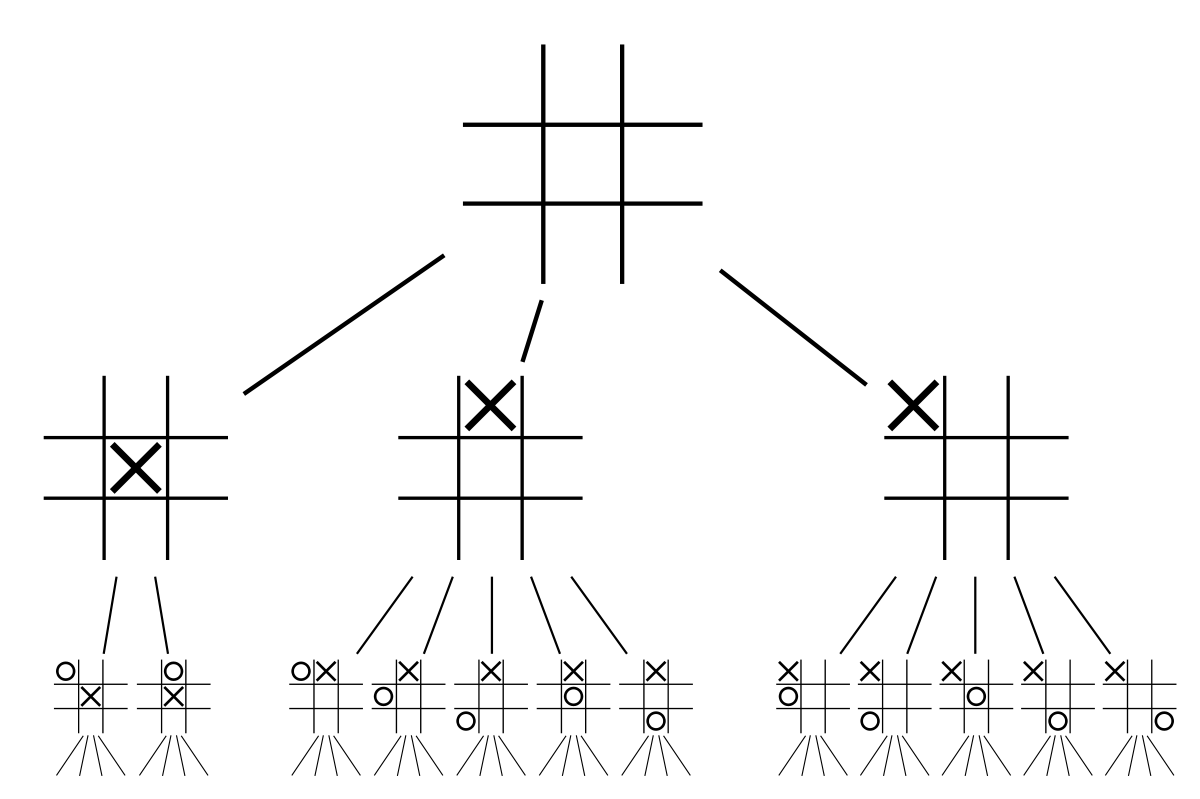
\includegraphics[scale=0.25]{tic-tac-toe-tree.svg.png}
\caption{Tic-Tac-Toe game tree from Wikipedia}
\end{figure}
In the game tree above, the nodes are game states and the edges are possible actions that players can take to move from one state to another. For two player games like Tic-Tac-Toe or Chess, the moving player alternates as we go down each level of nodes and edges. For an $n$-player game where players take turns in order, the levels would cycle through the players from $1$ to $n$. The root of the tree is the starting position we search from, in this case the beginning of the game.
\section*{Minimax}
Now that we know how states evolve, how can we figure out the best move? \\[0.2cm]
To simplify our analysis, we will focus on two-player \textbf{zero-sum} games. A two-player zero-sum game is one where \textbf{reward} values for players sum to $0$. A common class of zero-sum games are those where we reward the winning player $+1$ and the losing player $-1$ so that the sum of reards is $0$. \\[0.2cm]
In this setting, there is a very common algorithm for finding the best move that is known as \textbf{minimax}. After the first player moves, the second player wishes to maximize their reward from the new state. Sicne the game is zero-sum, the first player wishes to minimize the reward of the second player in order to maximize their own. Then the first player wishes to minimize the maximum reward that the second player can obtain after their move. Iterating this logic, the second player will want to maximize the minimum reward that they can get after the first player's next move. \\[0.2cm]
These alternating turns of minimizing and maximizing a reward function lead to the name minimax. The algorithm is also known as \textbf{maximin} if the first player instead maximizes and the second player minimizes but these are conceptually identical and are used interchangeably.
\newpage
\section*{Minimax Example}
\begin{table}[H]
\begin{center}
\begin{tabular}{|c|c|c|}
    \hline
    & $B$ Cooperates & $B$ Defects \\
    \hline
    $A$ Cooperates & 0 & -4 \\
    \hline
    $A$ Defects & -1 & -3 \\
    \hline
\end{tabular}
\end{center}
\caption{Rewards for Player $A$ in a Zero-Sum Game}
\end{table}
Next we will look at a simple example of how minimax can be applied to find the optimal move. Consider the game above between two players $A$ and $B$ where player $A$ moves first and each player can either cooperate or defect. The rewards for player $A$ are shown above and the rewards for player $B$ are the opposite values since the game is zero-sum. \\[0.2cm]
Now $A$ wants to decide what to do and knows $B$ will respond by picking the state with the minimum reward for $A$. If $A$ chooses to cooperate, $B$ will minimize over $\{0, -4\}$ and will choose to defect, leaving $A$ with $-4$. If $A$ instead chooses to defect, $B$ minimizes over $\{-1, -3\}$ and defects and $A$ receives a reward of $-3$. Since $A$ wants to maximize between these two options, A chooses to defect and gets a reward of $\max(\min(0, -4), \min(-1, -3)) = \max(-4, -3) = -3$. The alternating maxes and mins in this expression arise naturally from the competing goals of players $A$ and $B$.
\section*{Minimax Tree}
For larger games, the minimax algorithm is more easily visualized via a tree.
\begin{figure}[H]
\centering
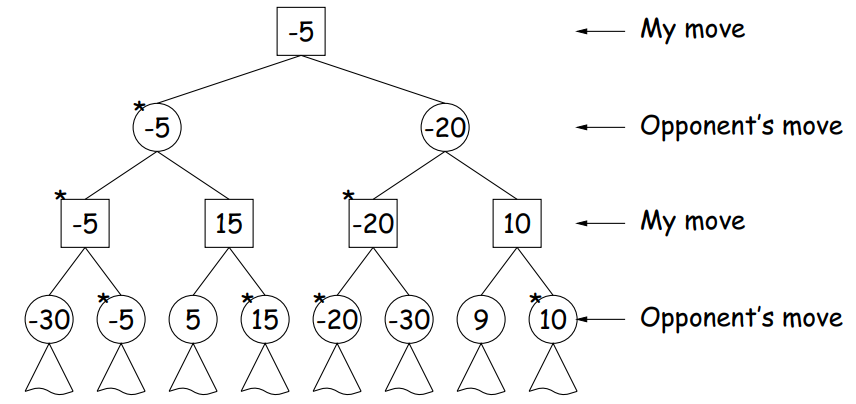
\includegraphics[scale=0.4]{minimax-tree.png}
\end{figure}
We begin with leaf nodes corresponding to ending game states with known reward. From these states, the rewards at the states one level above can be determined. At this level, you are the moving player so you look at the two child leaf nodes of each node and pick the one with maximum value. This yields the values $\max(-30, -5) = -5, \max(5, 15) = 15,\max(-20, -30) = -20,\max(9, 10) = 10$. At the level above this, it is your opponent's move and they minimize over the children of each node, yielding $\min(-5,15)=-5, \min(-20,10)=-20$. Finally at the top level, you calculate $\max(-5, -20) = -5$.
\newpage
This example illustrates how minimax can be used to evaluate intermediate game states. Furthermore, by storing the calculated optimal actions inside each node, you can easily execute the optimal strategy for a game. Due to the dependence of parent nodes on their child nodes, the minimax algorithm can be described via the following recursive procedure. \\[0.2cm]
\underline{Minimax Algorithm}
\begin{enumerate}
    \item If the game is over, return the value for this state.
    \item Otherwise, loop over each possible action.
    \item Execute the minimax algorithm on each of the resulting states with the opposite player to calculate their values.
    \item Return the action with maximum/minimum value if you are the maximizing/minimizing player.
\end{enumerate}
The games we have mentioned so far (Chess, Tic-Tac-Toe, the two games above) all are deterministic games. For stochastic games, there is an extension of minimax called \textbf{expectiminimax}, which instead minimizes/maximizes over the expected reward to choose actions and calculate expected rewards of earlier states. The reward function must be defined carefully with this algorithm. If reward for a checkers game was chosen to be number of leftover pieces, the algorithm would potentially maximize margin of victory at the cost of winning chances. In contrast, defining reward as $\pm 1$ for a win or loss would optimize winning probability. Expectiminimax is quite powerful and often performs well in the CS61A Hog Contest.
\section*{Heuristics}
The above method requires that we iterate over all game states starting from the ending states and building upwards. But this is computationally infeasible when there are too many states. For instance, the board game Othello has about $10^{28}$ states and a laptop computer wouldn't finish iterating over this many states before the end of the universe. \\[0.2cm]
To address this issue, we can cut off our tree at some depth and try to get a reasonable estimate of the values of nodes at this depth. Then we can simply apply minimax to this truncated tree to calculate the optimal actions based on our estimates. \\[0.2cm]
How can we get these estimated values of states? The function that is used to map from states to estimated values is called a \textbf{heuristic}, and will of course vary from game to game. Heuristics usually combine together various parameters of the state into estimates. For example a simple Tic-Tac-Toe heuristic might be $(\text{X's in a row}) - (\text{O's in a row})$ since we might expect the first player to be more likely to win if there are more X's and less likely to win if there are more O's. The problem of choosing such a heuristic is a good candidate for machine learning since it is effectively a regression problem and training data is easily obtained. \\[0.2cm]
Interestingly, minimax can itself be thought of as searching up to a given depth and then evaluating a heuristic function which happens to require searching further. This suggests that with a sufficiently good heuristic, searching up to a given depth can be almost as good as minimax. For moderately large games, this strategy can often outperform humans.
\newpage
\section*{Alpha-Beta Pruning}
Though heuristics allow us to come up with estimated values from limited depth searches, they do not address the issue of severely reduced search depth for larger games. A board state in Chess has about $35$ legal moves on average so the number of possible states increases exponentially with search depth. The number 35 is called the \textbf{branching factor} since each state branches out into $\sim 35$ new states. A search $6$ moves deep must consider $\sim 35^6 \approx 2$ billion moves which is already pushing the limits of a typical computer. Some good Chess players are able to see well beyond $6$ moves ahead, so how are computers able to vastly outperform the best players in the world? \\[0.2cm]
Aside from sophisticated evaluation functions, the answer is a more efficient search algorithm known as \textbf{alpha-beta pruning}. The key idea of alpha beta pruning is that we can can skip or "prune" a subtree if a player is guaranteed a better outcome by choosing a different action in some ancestor. In each state, we maintain two values $\alpha$ and $\beta$ which are the minimum and maximum values that players can achieve in the current state or its ancestors. If these values are updated so that $\beta < \alpha$, we will know that a player can achieve a better value in one of the ancestors and can prune this current state's subtree.
\section*{Alpha-Beta Pruning Example}
To gain more intuition, we demonstrate alpha-beta pruning with the same game tree as above.
\begin{figure}[H]
\centering
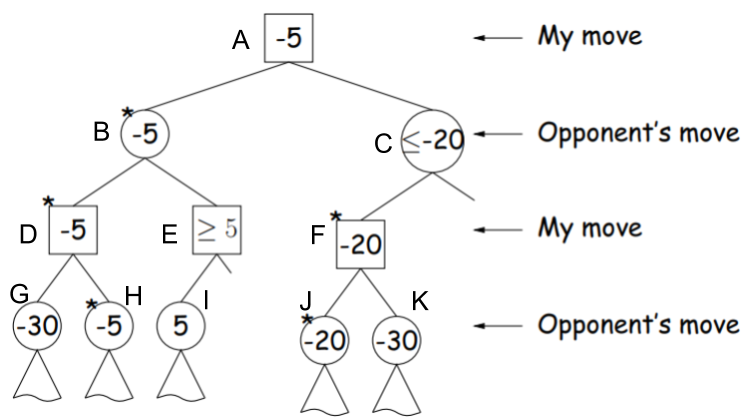
\includegraphics[scale=0.4]{alpha-beta.png}
\end{figure}
We begin from $A$ and initialize worst case values of $\alpha = -\infty, \beta = \infty$. We move left down the tree and reach $D$. At $D$, we first see $G$ has value $-30$. It is the maximizing player's turn so we update $\alpha = \max(-\infty, -30) = -30$. Then we see $H$, update $\alpha = \max(-30, -5) - -5$, and return $-5$. \\[0.2cm]
Now at $B$ the minimizing player can force a value of $-5$ by moving to $D$ so $\beta$ at $B$ is updated to $\min(\infty, -5) = -5$. We move to $B$'s right child, $E$, with this new $\beta$. Child $I$ has value $5$ so the maximizing player can achieve $\alpha = \max(-\infty, 5) = 5$ at $E$. However, $\beta < \alpha$ since the minimizing player can guarantee a lower value at $D$ so we prune $E$'s subtree and $B$'s value becomes $-5$. \\[0.2cm]
After $\alpha$ is updated to $-5$ at $A$, we move to the right subtree and find $F$ has value $\max(-20, -30) = -20$. The minimizing player can move to $F$ from $C$ so $\beta = \min(\infty, -20) = -20$ at $C$. However, $C$ was passed $\alpha = -5$ from $A$ and $\beta < \alpha$ since the maximizing player will always choose $-5$ over $-20$ at $A$. So $C$'s subtree is pruned and we find that the starting state $A$ has value $-5$. \\[0.2cm]
With alpha-beta pruning, we can search almost twice as deep as minimax in roughly the same time. \\[0.2cm]
The alpha-beta pruning algorithm can be summarized as follows. \\[0.2cm]
\underline{Alpha-Beta Pruning}
\begin{enumerate}
    \item If the current state is at our search depth limit or is an ending state, return its heuristic value.
    \item Otherwise, iterate over each possible action.
    \item For each of the resulting states, run alpha-beta pruning for the opposite player with the current $\alpha$ and $\beta$ values.
    \item Update $\alpha$ with the state value if you are the maximizing player or $\beta$ if you are the minimizing player.
    \item If $\beta < \alpha$ after updating, return the best action and exit.
    \item Otherwise, if the current action has better value than the best action so far, update the best action.
    \item After the iteration is finished, return the best action.
\end{enumerate}
\section*{Iterative Deepening}
In practice, we usually want the computer to calculate a reasonable move in some fixed amount of time. We could easily do this if we knew how long it would take to search at a given depth. But this can vary based on the branching factor of the game at various points and how often we are able to prune using alpha-beta pruning. Furthermore, it's important to finish searching at a given depth before searching deeper. Otherwise, we could be searching suboptimal moves very deeply while neglecting the best move in another part of the tree. \\[0.2cm]
An initial approach that you might come up with is breadth first search. Since this search gradually increases depth, we could keep searching deeper and deeper until time runs out and then return the best move at the highest depth we have finished searching. Unfortunately, breadth first search requires that the previous level of nodes is stored in a queue and the number of nodes in a level increases exponentially so we will quickly run out of memory. Furthermore, alpha beta pruning involves searching one subtree deeper in order to bound state values and avoid searching other subtrees. But if we are only increasing depth by $1$ each iteration, there is little opportunity for this. \\[0.2cm]
An idea of \textbf{iterative deepening} is used to resolve this issue. We start by running a search at a small depth like $d = 1$ and keep rerunning the entire search, increasing $d$ by $1$ each time. If we use depth first search for this, our memory is only the $O(d)$. This might seem extremely inefficient - why are we redoing all of our previous work every time we search? \\[0.2cm]
Surprisingly, since the number of nodes in a game tree usually increases exponentially at each level, all of the previous search times become negligible compared to the search time for the last level for a sufficiently large branching factor. Iterative deepening ends up having the same asymptotic runtime as breadth first search while having vastly better space and using alpha-beta pruning on each individual search. As a result, iterative deepening allows for adaptable game engines that can perform well in time-limited settings.
\end{document}